% A simple LaTeX template for lab reports in TDT4258 Energy Efficient Computer Design
% by Yaman Umuroglu (yamanu@idi.ntnu.no)
% Feel free to customize the style as you see fit, but the chapters/sections mentioned in the
% template should be included with the appropriate content.

\documentclass[abstract=on]{scrreprt}
\usepackage[utf8]{inputenc} % allow utf-8 characters

\usepackage[T1]{fontenc}    % angle brackets in text mode

\usepackage{natbib}         % bibliography management
\usepackage{graphicx}       % images

\usepackage{listings}       % source code listings
\usepackage{hyperref}       % hyperlinks
\usepackage{url}            % the \url command
\usepackage[all]{hypcap}    % follow links to captions correctly

\usepackage{amsmath}		% for advanced mathematics

\usepackage{float}		% hard floating specifier
\usepackage{verbatim}	% multiline comment support

% Edit the meta.tex file to change title, group number and author names
% Fill in the report title, group number and student names here
\newcommand{\mytitle}{Energy efficient LED controller}
\newcommand{\mygroupnumber}{24}
\newcommand{\myauthor}{Peter Aaser\\Audun Sutterud\\Jonatan Lund}

% Appearance of source code listings
% TODO: Adapt this to assembly
\usepackage{color}
\definecolor{mybgcolor}{rgb}{0.9, 0.9, 0.9}
\definecolor{mycommentcolor}{rgb}{1.0, 0.0, 0.0}
\definecolor{mykeywordcolor}{rgb}{0.58,0,0.82}
\definecolor{mystringcolor}{rgb}{0.9,0.5,0.15}
\lstset{
    language=C,
    backgroundcolor=\color{mybgcolor},      % set background color
    frame=single,                           % draw border
    basicstyle=\ttfamily,                   % font
    commentstyle=\color{mycommentcolor},    % styles
    keywordstyle=\color{mykeywordcolor},    %
    stringstyle=\color{mystringcolor},      %
    breakatwhitespace=true, % break lines if necessary
    breaklines=true,        %
    tabsize=4,              % indentation size
    columns=flexible,       % preserve indentation
    keepspaces=true,        %
    morekeywords={as},      % additional keywords
    captionpos=b,           % place captions below listing
}

\title{\mytitle}
\author{\myauthor}
\date{\today}



\begin{document}
% The title page, edit if you want to customize it
\begin{titlepage}

\includegraphics[height=1.5cm]{images/ntnu_logo.pdf}\\[1cm]   
\begin{center}

 
% Upper part of the page
~\\[1.5cm]

\textsc{\Large TDT4258 Energy Efficient Computer Design\\Laboratory Report}\\[0.5cm]

% Set the title of the Document between two horizontal lines
\hrule ~\\[0.2cm]
{\huge \bfseries \mytitle}\\[0.4cm]		% print the title of the document
\hrule ~\\[1.5cm]

% Additional Information about the document
\begin{minipage}{0.4\textwidth}
    \centering
	\large
		\emph{Group \mygroupnumber:}\\~\\
		\myauthor
\end{minipage}

\vfill

% Bottom of the page
{\large \today}

\end{center}
\end{titlepage}


% Main matter - edit corresponding file under content/ to change
\begin{abstract}
In this exercise we have explored basic features of the EFM32GG-DK3750 development kit, including how to connect it to a computer for loading code and monitoring its state, how to interface with it via a prototype gamepad, and how to monitor energy efficiency of our programs with EnergyAware Profiler. On the development end we learned how to use a toolchain for compiling and loading files onto the microcontroller, how to use the GNU Debugger with GDBServer to debug running code, some basic ARM assembly for the Cortex-M3 microprocessor and how to control the rest of the board by writing and reading memory.

To do this we have implemented a small program mapping buttons to LEDs, first with a simple polling loop, then with a more sophisticated interrupt based program, and lastly a simple countdown clock.
\end{abstract}

\tableofcontents
\chapter{Introduction}
% Your report should start with an introduction chapter that motivates the subject in general and describes the problem you are trying to solve.

Embedded computing systems are being deployed on an increasingly larger scale, and it is expected that this trend will continue in the forseable future. It follows that there is a great market for developing software for embedded computing systems. In contrast to general-purpose computing, embedded computing often places strong constraints on energy consumption, performance, and cost. In order to implement these qualities in a system, software developers must make extensive use of low-level hardware functionality, and specific knowledge of the hardware components and technology used is required. 

The course TDT4258 Energy Efficient Computer Systems gives an introduction to microcontroller programming on a practical and theoretical level, with a strong focus on energy-efficiency. Through lectures and three comprehensive exercises the students get theoretical knowledge as well as hands-on experience. The development platform used is the EFM32GG-DK3750 development kit from Silicon Labs, and the tools used include energyAware Commander and the GNU Compiler Collection.

In the first exercise we will connect the prototyping board to a specially built gamepad with LEDs and buttons, and write a small program that lets the user to control the gamepad LEDs through the buttons. The purpose of the exercise is to introduce the development kit hardware, to become familiar with writing low-level energy-efficient software, and to learn software development using the GNU-toolchain. All code will be written in assembly using the Thumb-2 instruction set, and no operating system will be running. An important exercise goal is that the program should be energy-efficient, and thus we need to utilize low-level hardware functions to improve the power consumption. To learn different techniques to improve the power consumption, we are encouraged to read the relevant reference manuals and data sheets. 


\chapter{Background and Theory}
% This chapter should describe the theoretical background needed to understand
% and solve the problem. For instance, a description of the hardware platform
% or specific components involved in this assignment, definition of concepts
% that are important to understand the solution should be summarized here. Add
% citations to show sources whenever appropriate, LaTeX and bibliography
% managers make this easy.

% TODO: Write an introduction to ptxdist usage


\section{Operating Systems}
An operating system is a special piece of software that provides two important functions in a computer:
\begin{itemize}
  \item Managing the hardware resources.
  \item Providing a useful hardware abstraction layer for application programmers.
\end{itemize}
The core of the operating system is called the \emph{kernel} and runs in a privileged software mode that gives the kernel complete access to all hardware resources. The code running outside the kernel is often referred to as the \emph{user space} or the \emph{userland}, and has only restricted access to hardware. Because of this organization, all hardware-related activities necessary to run the operating system is performed by the kernel, and the user space programs only access hardware through \emph{system calls} in the kernel.\cite{modern-operating-systems}

\subsection{Device Driver}
To more easily manage hardware devices with different characteristics, the kernel contains \emph{device drivers}. A device driver is a program that manages low-level hardware access to a particular device, providing a clean interface for the rest of the kernel programs.

\subsection{Kernel Module}
It is sometimes necessary to extend the functionality of the kernel, for instance if new hardware becomes available. While this could be achieved by modifying and rebuilding the kernel, a much more attractive alternative is to use \emph{kernel modules}, small programs that are loaded at runtime and extend the kernel with the needed functionality. Device drivers can be added as kernel modules.
% TODO: Write a brief explaination on OS terminology.


\chapter{Methodology}
This chapter details the methods used and the process with which we achieved our results.

\section{Process Overview} %Introductory chapter, sort of

\subsection{Exercise Description}
The goal of this exercise was to write a program for the EFM32GG that generated sounds by utilizing the onboard Digital to Analog Converter. The program should make at least three different sound effects, as well as a melody. These should be appropriate for use in the final exercise of the course where the goal is to create a game, and it should be possible to control which sound is being played by pressing the different buttons of the prototype gamepad. The program should be written in C, and should run directly on the EFM32GG hardware with no operating system involved. Emphasis was placed upon energy efficiency, an energy efficient solution will be rewarded with extra points.

TODO % Write something about the rest of the approach


\section{Initial Approach}
In order to get an introduction to programming the DAC we created a program intended to play a single continuous note. This would be an easy introduction to C programming, and would give us a good performance baseline with regards to energy consumption.

\subsection{GPIO Setup} 
The first step was porting the assembly code we had previosuly written to control LEDs and clocks over to C. Having set up the LEDs and buttons would also make it easier to debug the code by writing values to the LEDs to discern the current program state. Rather than starting with a simple polling loop we felt confident enough to go straight to interrupts for the LEDs and buttons, letting the program idle in a loop between interrupts.

The code we used to set up the GPIO pins for input and output is shown in code listing \ref{lst:gpio-setup1} and \ref{lst:gpio-setup2} respectively. In addition to the steps shown, the clock signal for the modules needed to be enabled in the CMU. \\

\noindent\begin{minipage}[pos=c,contentpos=c]{\textwidth}
  \begin{lstlisting}[caption=Setting GPIO pins 0-7 as input,label={lst:gpio-setup1}]
  *GPIO_PC_MODEL = 0x33333333;  // Set pins 0-7 as input pins
  *GPIO_PC_DOUT = 0xff;         // Enable pull-up resistors
  *GPIO_EXTIPSELL = 0x22222222; // Set interrupt generation for pin 0-7
  *GPIO_EXTIFALL = 0xff;        // Set interrupt on 1->0
  *GPIO_EXTIRISE = 0xff;        // Set interrupt on 0->1
  *GPIO_IEN = 0xff;             // Enable interrupt generation
  \end{lstlisting}
\end{minipage}

\noindent\begin{minipage}[c]{\textwidth}
  \begin{lstlisting}[caption=Setting GPIO pins 8-15 as output,label={lst:gpio-setup2}]
  *GPIO_PA_MODEH = 0x55555555; // Set pins 8-15 to output
  *GPIO_PA_CTRL = 2;           // Set high drive strength
  \end{lstlisting}
\end{minipage}


\subsection{DAC Setup}
The setup code we wrote for the DAC closely followed the instructions in the compendium, as shown in code listing \ref{lst:dac-setup}. With this setup, the DAC would continuously read both its 12 bit channels and update the output voltage. The next step to generate sound was to continously write samples to the channels emulating an audible waveform.\\

\noindent\begin{minipage}[c]{\textwidth}
  \begin{lstlisting}[caption=Setting up the DAC,label={lst:dac-setup}]
  *DAC0_CTRL = 0x50000; // Set a DAC clock division factor of 32
  *DAC0_CTRL |= 0x10;   // Set continuous mode
  *DAC0_CH0CTRL = 1;    // Enable left channel
  *DAC0_CH1CTRL = 1;    // Enable right channel
  \end{lstlisting}
\end{minipage}

\subsection{TIMER setup}
We chose to base our initial implementation on interrupts, writing a new sample to the DAC whenever an interrupt occurred. The sampling rate could then be set by setting the frequency of the interrupts. To generate interrupts, we used the TIMER module, setup as described in listing \ref{lst:timer-setup}. Note the variable \texttt{period} used to set interrupt frequency. \\

\noindent\begin{minipage}[c]{\textwidth}
  \begin{lstlisting}[caption=Setting up the timer to generate interrupts,label={lst:timer-setup}]
  *TIMER1_TOP = period; // Set period between interrupts
  *TIMER1_IEN = 1;      // Enable interrupt generation
  *TIMER1_CMD = 1;      // Start the timer
  \end{lstlisting}
\end{minipage}

Finally, an interrupt handler was written that used a simple conditional statement to write a square waveform to the DAC channels, oscillating the DAC voltage between 0 and 1000. Our first attempt was outside of the audible frequency range, but by adjusting the timer we could reduce the amount of interrupts to control the frequency.


\section{Efficient Interrupts}
After setting up everything we needed to generate a simple tone we decided to do some preliminary optimizations in our program. Rather than using the TIMER module we would use the LETIMER with a max speed of 32678 Hz, more than ample for our needs. As the LETIMER module was available in EM2 and EM3, this would allow us to potentially save energy by entering EM2 between the interrupts. \\

% and turning off the HF clock between samples.

\subsection{LETIMER and LFACLK Setup}
As the LETIMER is driven by the LFACLK clock, we needed to configure the LFACLK clock before using the LETIMER. The LFACLK was configured using the code shown in listing \ref{lst:lfaclk-setup}, and the LETIMER was configured using the code shown in listing \ref{lst:letimer-setup}. 

\subsubsection{Choosing Low Frequency Oscillator}
To drive the LFACLK we had the choice of either using the Low Frequency Crystal Oscillator (LFXO) or the Low Frequency RC Oscillator (LFRCO). After some initial testing we found that the LFRCO was unstable due to temperature differences, producing a slight variation in the pitch of the generated sound. LFXO was stable enough for our purposes. However, it had a longer start-up time, and we were aware that it might introduce delays into our program when waking up from low energy modes. \cite{efm32-oscillator-design-considerations-application-note} \\
 
\noindent\begin{minipage}[c]{\textwidth}
  \begin{lstlisting}[caption=Setting up the LFACLK to drive the LETIMER ,label={lst:lfaclk-setup}]
  *CMU_OSCENCMD |= (1 << 8);    // Start the LFXO
  *CMU_LFCLKSEL &= ~(0x3 << 0); // Select LFXO to drive LFACLK
  *CMU_LFCLKSEL |= (2 << 0);    //
  *CMU_LFACLKEN0 |= (1 << 2);   // Enable clock signal for LETIMER 

  // Enable clock for the Low Energy Peripheral Interface
  *CMU_HFCORECLKEN0 |= (1 << 4);
  \end{lstlisting}
\end{minipage}

\noindent\begin{minipage}[c]{\textwidth}
  \begin{lstlisting}[caption=Setting up LETIMER to generate periodic interrupts,label={lst:letimer-setup}]
  *LETIMER0_CTRL |= (1 << 9); // Set period between interrupts
  *LETIMER0_COMP0 = period;   // 
  *LETIMER0_CMD |= (1 << 0);  // Start the LETIMER
  *LETIMER0_IEN |= (1 << 2);  // Enable interrupt generation
  \end{lstlisting}
\end{minipage}


\section{Generating Songs}
We decided early in the process that we wanted to use the EFM32GG to play songs. We explored several different methods to create songs with the EFM32GG, and eventually decided on two different approaches. In the first approach, pre-synthesized samples were loaded on to the board at compile time. In the second approach, distinct notes coded as 16 bits words were loaded on to the board at compile time, and then synthesized at run-time by a software synthesizer. The result was two different implementations: The \emph{on-board synthesizer} and the \emph{sample-based music player}, described in section \ref{sec:onboard-synthesizer} and \ref{sec:sample-based-music-player} respectively.

\subsection{Memory Limitations}
The EFM32GG board has 128 kB of SRAM and 1024 kB of flash memory. This puts limitations on how a song is stored in the memory on the EFM32GG. Considering stoting the samples of a song sampled at 44100 Hz where each individual sample is 2 bytes large and the song duration is $d$ seconds. The size of the song can be calculated with the formula
$$\text{Song size (bytes)} = 88.2 \cdot d$$.
To find the longest song with a size that will fit in SRAM, we set $88200d = 128 kB = 131072 B$ which yields $d = 1.49$. Thus the longest song that will fit in SRAM is shorter than 1.5 seconds! This can be remedied somewhat by choosing a lower sample rate and possibly utilizing flash memory, but the EFM32GG will be hard pressed to store any quality song much longer than 30 seconds. Our two approaches uses different techniques to evade the memory limitations.

\subsection{On-board Synthesizer}\label{sec:onboard-synthesizer}
To overcome the memory limitations, this implementation uses the EFM32GG as a synthesizer to generate square waveforms. A song is stored in memory as integer arrays. The integer array contains information to create different tones. Two integer arrays produces a song with two channels.

Our first thought was to save all the samples of a song. 

\subsubsection{Song Representation}
In our solution we chose to represent a song as an array of 16 bit int values. These arrays is generated by a python script and placed in the source code. Inside these 16 bits we store information about pitch, octave, amplitude and duration. In table \ref{tab:bitFields} the bit partitions are described.

\begin{table}[H]
	\begin{center}
	\begin{tabular}{ |c|c|c|c| }
	  \hline
	  Duration & Amplitude & Octave & Pitch \\
	  \hline
	  5 & 3 & 4 & 4 \\
	  \hline

	\end{tabular}
	\caption{Bit partitioning}
	\label{tab:bitFields}
	\end{center}
\end{table}

Each pitch value is represented by a value from 0 to 11. The Octave can take the values 0-10. Note A with octave 0 is lowest possible at 27.5 Hz, and note A with octave 10 the highest at 28160 Hz. DAC's lowest values is to low hear, beacuse of this we calculated the amplitude with the equation \ref{eq:amplitudCalculation}. In addition we only had 3 bit to store the amplitude values, and as a result we calculated it exponentially. Duration takes values between 0-32. In our program we define the duration of the shortest note. The duration value is multiplied with the defined duration value and returns each notes duration given in milliseconds. By changing the defined duration value we can increase or decrease the song's speed.

\begin{equation}
  x = 2^{amplitude + 5}
  \label{eq:amplitudCalculation}
\end{equation}

\subsubsection{Song Playback}
To play a song the synthesizer wakes up 32768 times every second. Each tone is played with square waves. After calculating each tone's frequency the synthesizer turns the DAC on and off, to match the tone frequency. This method has limitations when it comes to reproducing sounds, but this metod is very space efficient.


\subsection{Sample Based Music Player}\label{sec:sample-based-music-player}
An issue with the synth is that in order to generate more advanced waveforms a program must utilize expensive trigonometric calculations to express them. Although the EFM32GG does have the capability to generate a sine wave on the DAC, in order to play actual music a more advance approach is required. To achieve this we decided to do the expensive calculations on a personal computer, using a synthesizer to sample a sine wave and output an array that could be compiled. Although the limited DAC sound quality made it possible to use a fairly low sample rate with no discernable quality difference we settled on using the maximum sample rate the LFXO clock could grant us, 32768 samples per second. 

\subsubsection{Song Representation}
In order to play back sound at a given sample S with B bits accuracy the required data is S*B per second. for 12 bits accuracy at a 32768 samples per second that equates 48kB for a second of music, unfeasible for the 128kB of SRAM the EFM32GG has. Additionally, in order to simplify access to sample the 12 bit values would be loaded into 2 bytes, effectively making each 12 bit sample take 16 bits of storage. In order to save space we therefore decided to create samples of the frequencies we needed into short segments that could be repeated as long as we wanted the sound to play. To implement this idea we created an array with 100 sample pointers as a lookup table for notes, where every note was assigned its own number, initializing only the pointers that pointed to a note that would be played. A song could then be encoded as an array of instructions to access various notes and repeat the sample for a set duration.


\begin{figure}[ht]
  \centering
  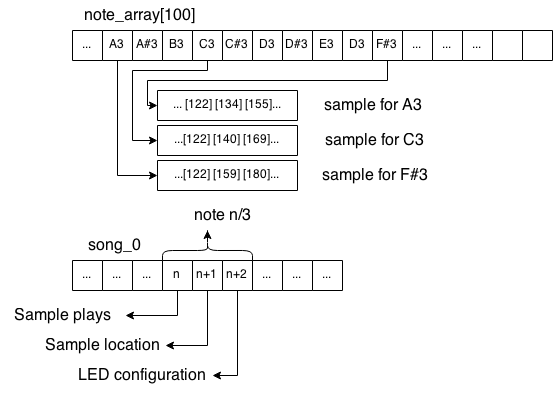
\includegraphics[width=\textwidth]{images/sample_array_layout.png}
  \caption{A map of the memory layout for the sample based approach}\label{fig:array_layout}
\end{figure}

\noindent\begin{minipage}{\textwidth}
\begin{lstlisting}
typedef struct Player
{
	uint16_t song;			// Number of current song
	uint16_t song_len;		// Total notes for current song
	uint16_t notes_played;	// Keeps track of notes
	uint16_t sample_total;	// Times current sample should play	
	uint16_t sample;		// Times current sample has played
	uint16_t sample_i;		// Position in current sample 
	uint16_t note_len;		// Length of current sample
	uint16_t* note;			// Location of current sample
	uint16_t LED;			// Current LED configuration
} Player;
\end{lstlisting}
\end{minipage}

\subsubsection{Song Playback}
In order to play a song we bundled the necessary attributes to keep track of what notes to play and their tempo together in a Play struct. To initialize a song play\_init() is called with the song to be played as the argument. This sets up a playback. After initializing calling the play() function will output the next sample to the DAC.
The play() function keeps track on the current position of a playback, reading from an array of triplets to load the next note whenever the current one has been finished.

\noindent\begin{minipage}{\textwidth}
\begin{lstlisting}
void play(void){
	// Load the next sample
	if(player.sample_i < player.note_len-1){			
		player.sample_i++;								
	}
	else{								
		player.sample_i = 0;
		if(player.sample < player.sample_total){
   			player.sample++;				
		}
		else{							
			player.sample = 0;
			if(player.notes_played < player.song_len){
				next_note();
				(*GPIO_PA_DOUT) =  player.note_len << 8 ;		
			}			 
			else{
			  disableLETIMER();
			  disableDAC();
			  //__asm("wfi");
			}
		}
	}
	// Write the sample to the DAC
	*DAC0_CH0DATA = player.note[player.sample_i];
	*DAC0_CH1DATA = player.note[player.sample_i];
}
\end{lstlisting}
\end{minipage}

\section{The Final Program}
In order to string together our different approaches to a single coherent program we made a sound selector using the GPIO functionality. Different sounds were mapped to different buttons such that pressing a mapped button would start a song. In addition we wrote functionality to toggle the LETIMER and DAC on and off, as well as toggling different sleep behaviour and switching between synth and sample playback. By necessity we also implemented a silencing function to make the board stop playing and power down extra functionality.

\section{Optimization}
In order to reduce energy consumption we had two areas to focus on, efficiency when playing and standby mode. In order to make the board go back to sleep after finishing a playback or being manually halted we implemented several toggle functions in order to put the board to sleep when not used. When actively playing we tried different energy modes to observe whether maintaining the cache in EM1 would lead to greater energy efficiency compared to going down to EM2, effectively flushing the cache.

\subsection{Sleeping Between Interrupts}



\section{Testing}
In order to test the functionality of our program we relied on visual and aural feedback rather than software approaches such as GDB. By using the LEDs we could write values directly to the LEDs, and with the earphones we could hear whether the sound was playing correctly or not. In order to measure energy consumption we used the onboard LCD screen for quick estimates. For higher quality measurements we used eAProfiler on a PC to read energy consumption on the board via the USB connection. We performed all final measurements in succsession on a board that had been in use for several hours to minimize measurement variance. 

\chapter{Results}
TODO
% In this chapter, you should discuss the results you have obtained from your
% implementation. These can be correctness results, i.e whether the
% implementation behaved as expected, or numerical results that express runtime
% or energy measurements.

\section{Energy Modes}
\label{sec:energyModeResults}
While a song is playing the board consumes a significant amount of power. To decrease the consupmtion, we tried different energy modes between interrupts. We measured energy consumption in EM0, EM1 and EM2. The results can be seen in table \ref{tab:benchmarkEnergyModes}. In our case EM1 gave best results and not EM2 as first expected.

\begin{table}[ht]
	\begin{center}
	\begin{tabular}{ |c|c|c| }
	  \hline
	  EM0 & EM1 & EM2 \\
	  \hline
	  4.85 mA & 4.02 mA & 4.51 mA \\
	  \hline

	\end{tabular}
	\caption{Energy consumption with different energy modes}
	\label{tab:benchmarkEnergyModes}
	\end{center}
\end{table}

\section{Song Size}
In order to compare the two implementations we needed to not only compare efficiency but also utility. 

\subsection{Synth Songs}
The synth based approach yielded fairly small song sizes, the tetris theme totalled at 204 bytes, needing only two arrays of respectively 38 and 64 16 bit integers. With this size we could fit in a lot of music before size would become an issue.

\subsection{Samples}
For the sample based apprach we used samples averaging at around 1640 integers per array for 0.05 seconds. Clearly the samples were a lot more memory intensive. While sample size could be brought down by only sampling a single waveform we decided 0.05 second samples would be more interesting to work with since they would allow for variance in the waveforms, creating more interesting tones. The final size per sample ended up averaging around 3280 bytes, a significant cost compared to the synth approach. However, reuse of samples can offset this cost somewhat since playing a note twice comes at the same cost as the synth approach

\chapter{Conclusion}
In this exercise we have compiled an OS and implemented the necessary drivers to interact with the board via a gamepad. 

On these foundations we have developed a fairly complex game running in real time with a lot of calculations, taxing the recourses of the board heavily. Even with the relatively large demands of our game, and the added overhead of running an operating system, we have shown that hitting 30 frames per second with a fairly complex vector based game is possible.

\section{Evaluation of the Assignment}
% You can include comments about the assignment itself here. While this part is
% not obligatory and not graded, it is valuable feedback to the course staff
% that can be used to improve the exercises in the future.

\subsection{Compendium Feedback}
This section contains feedback and suggested improvements for the compendium.

\subsubsection{Mention \texttt{ptxdist clean} in section 5.3.3}
As mentioned in the compendium in section \textbf{5.3.3. Building and Flashing}, a single package can be flashed with the following four commands:
\begin{enumerate}
  \item \texttt{ptxdist compile <packagename>, e.g game or driver-gamepad}
  \item \texttt{ptxdist targetinstall <packagename>}
  \item \texttt{ptxdist image root.romfs}
  \item \texttt{ptxdist test flash-rootfs}
\end{enumerate}
However, in order for the modified sources to be compiled, we also needed run one of the commands \texttt{ptxdist clean game} and \texttt{ptxdist drop game compile}. Maybe it would be useful to mention this in this section.




% Bibliography - edit references.bib and use the \cite command in text
\bibliographystyle{plain}
\bibliography{references}
\end{document}
